\subchapter
{Root filesystem construction}
{Objectives:
  \begin{itemize}
  \item Explore the build output
  \item Customize the root filesystem using a {\em rootfs overlay}
  \item Customize the kernel with patches and additional configuration
    options
  \item Add more packages
  \item Use {\em defconfig} files and {\em out of tree} build
  \end{itemize}
}

\section{Explore the build output}

Now that we have discussed during the lectures the organization of the
Buildroot {\em output} tree, take some time to look inside
\code{output/} for the different build artefacts. And especially:

\begin{itemize}

\item Identify where the cross-compiler has been installed.

\item Identify where the source code for the different components has
  been extracted, and which packages have been built.

\item Identify where the target root filesystem has been created, and
  read the \code{THIS_IS_NOT_YOUR_ROOT_FILESYSTEM} file.

\item See where the \code{staging} symbolic link is pointing to.

\end{itemize}

\section{Configure the network on your host}

In the next sections of this lab, we will want to interact with the
BeagleBone Black over the network. So in this section, we'll configure
an Ethernet interface on your host machine.

With a network cable, connect the Ethernet port of your board to the
one of your computer. If the main wired Ethernet port of your computer
is already used, your instructor will provide you with a USB Ethernet
adapter. A new network interface, probably \code{eth1} or \code{eth2},
should appear on your Linux system.

To configure this network interface on the workstation side, click on
the {\em Network Manager} tasklet on your desktop, and select {\em
Edit Connections}.

\begin{center}
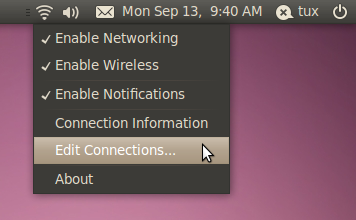
\includegraphics[width=8cm]{labs/buildroot-rootfs/network-config-1.png}
\end{center}

Select the new {\em wired network connection}:

\begin{center}
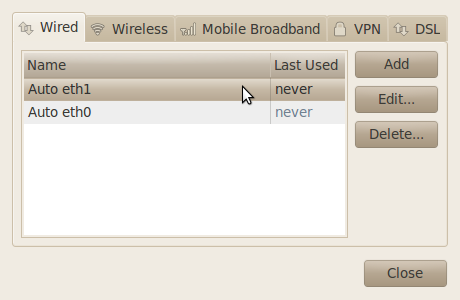
\includegraphics[width=8cm]{labs/buildroot-rootfs/network-config-2.png}
\end{center}

In the \code{IPv4 Settings} tab, press the \code{Add} button
and make the interface use a static IP
address, like \code{192.168.0.1} (of course, make sure that this
address belongs to a separate network segment from the one of the main
company network).

\begin{center}
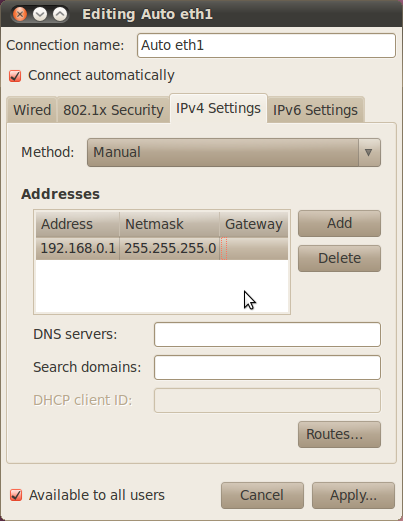
\includegraphics[width=8cm]{labs/buildroot-rootfs/network-config-3.png}
\end{center}

You can use \code{255.255.255.0} as \code{Netmask}, and leave the
\code{Gateway} field untouched (if you click on the \code{Gateway} box, you
will have to type a valid IP address, otherwise you won't be apply to
click on the \code{Apply} button).

{\em Note: using \code{ifconfig} in the command line is not
recommended, because Network Manager will unconfigure and reconfigure
the network interface each time the cable is unplugged or each time
the board reboots.}

\section{Add {\em dropbear} as an SSH server}

As a first additional package to add to our system, let's add the {\em
dropbear} SSH client/server. The server will be running on the
BeagleBone Black, which will allow us to connect over the network to
the BeagleBone Black.

Run \code{make menuconfig}, and enable the \code{dropbear}
package. You can use the search capability of \code{menuconfig} by
typing \code{/}, enter \code{DROPBEAR}. It will give you a list of
results, and each result is associated with a number between
parenthesis, like \code{(1)}. Then simply press \code{1}, and
\code{menuconfig} will jump to the right option.

After leaving \code{menuconfig}, restart the build by running
\code{make}.

In this case, we do not need to do a full rebuild, because a simple
\code{make} will notice that the \code{dropbear} package has not been
built, and will therefore trigger the build process.

Re-extract the root filesystem tarball in the \code{rootfs} partition
of the SD card. Don't forget to replace the entire root filesystem:

\begin{verbatim}
rm -rf /media/<user>/rootfs/*
sudo tar -C /media/<user>/rootfs/ -xf output/images/rootfs.tar
\end{verbatim}

Now, boot the new system on the BeagleBone Black. You should see a
message:

\begin{verbatim}
Starting dropbear sshd: OK
\end{verbatim}

Log in the system, and configure an IP address manually by doing
\code{ifconfig eth0 192.168.0.2}. Now, from your host machine, you can
connect over the network to the board by doing \code{ssh
root@192.168.0.2}.

However, configuring the IP address every time you boot the board is
not very practical, so let's move to the next section, in which we
will learn how to do this properly.

\section{Use a {\em rootfs overlay} to configure the IP address}

By default, Buildroot uses the \code{ifup} program from Busybox, which
reads the \code{/etc/network/interfaces} file to configure network
interfaces.

So, we could write a \code{/etc/network/interfaces} file on our
target, and reboot. However, the next time we will fully rebuild and
reflash our system, such changes will have disappeared. It is
important that our build process remains fully reproducible, so we
want to ensure that the next build will include such custom
configuration.

To achieve this, the easiest way is to use the {\bf rootfs overlay}
mechanism of Buildroot. Since this {\em overlay} is specific to our
project, we will create a custom directory for our project within the
Buildroot sources: \code{board/felabs/beagleboneblack/}.

Within this directory, create a \code{rootfs-overlay} directory, and
in \code{menuconfig}, specify
\code{board/felabs/beagleboneblack/rootfs-overlay} as the {\em rootfs
overlay} (option \code{BR2_ROOTFS_OVERLAY}).

Then, in \code{board/felabs/beagleboneblack/rootfs-overlay}, create a
file named \code{etc/network/interfaces} with the following contents:

\begin{verbatim}
auto lo
iface lo inet loopback

auto eth0
iface eth0 inet static
      address 192.168.0.2
      netmask 255.255.255.0
\end{verbatim}

Then, rebuild your system by running \code{make}. Here as well, we
don't need to do a full rebuild, since the {\em rootfs overlays} are
applied at the end of each build. You can check in
\code{output/target/etc/network/interfaces} if the contents of the
file are good.

Reflash the root filesystem on the SD card, and boot your BeagleBone
Black. It should now have an IP address configured for \code{eth0} by
default.

\section{Linux kernel customization}

Now, we would like to connect an additional peripheral to our system:
the {\em Wii Nunchuk}. Using this custom peripheral requires adding a
new driver to the Linux kernel, making changes to the Device Tree
describing the hardware, and changing the kernel configuration. This
is the purpose of this section.

We will first create a new directory to store our kernel patches. It
will sit next to our {\em rootfs overlay} in our project-specific
directory:

\begin{verbatim}
mkdir board/felabs/beagleboneblack/linux-patches/
\end{verbatim}

Copy in this directory the two patches that we provided with the data
of this lab, in \code{$HOME/felabs/buildroot-rootfs/}, but change
their name so that their start with \code{linux-}\footnote{Note: this
  renaming will no longer be necessary starting from Buildroot
  2015.05, all \code{*.patch} files will be applied.}:

\begin{verbatim}
cp $HOME/felabs/buildroot-rootfs/0001-.....patch \
     board/felabs/beagleboneblack/linux-patches/linux-0001-.....patch
cp $HOME/felabs/buildroot-rootfs/0002-.....patch \
     board/felabs/beagleboneblack/linux-patches/linux-0002-.....patch
\end{verbatim}

The first patch adds the driver, the second patch adjusts the Device
Tree. Feel free to look at them. If you're interested, you can look at
our training course {\em Embedded Linux kernel driver development},
which precisely covers the development of this driver.

Now, we need to tell Buildroot to apply these patches before building
the kernel. To do so, run \code{menuconfig}, go the to the {\em
Kernel} menu, and adjust the \code{Custom kernel patches} variable to
\code{board/felabs/beagleboneblack/linux-patches/}.

Let's now clean up completely the \code{linux} package so that its
sources will be re-extracted and our patches applied the next time we
do a build:

\begin{verbatim}
make linux-dirclean
\end{verbatim}

If you check in \code{output/build/}, the \code{linux-4.0} directory
will have disappeared.

Now, we need to adjust our kernel configuration to enable the {\em Wii
Nunchuk} driver. To start the Linux kernel configuration tool, run:

\begin{verbatim}
make linux-menuconfig
\end{verbatim}

This will:

\begin{itemize}
\item Extract the Linux kernel sources
\item Apply our two patches
\item Load the default kernel configuration
  \code{omap2plus_defconfig}, as we specified in the previous lab
\item Start the kernel \code{menuconfig} tool
\end{itemize}

Once in the kernel \code{menuconfig}, search for the option
\code{CONFIG_JOYSTICK_WIICHUCK} by using the search engine tool
accessible by typing \code{/}. Make sure to enable the {\em Nintendo
  Wiimote Extension connector on i2c bus} option using a \code{*} so
that the driver is part of the kernel image itself (enabling with
\code{M} would lead the driver to be compiled as a module). Also, make
sure the \code{CONFIG_INPUT_EVDEV} option is enabled with \code{*} (by
default it is enabled as a module).

You can now exit the kernel \code{menuconfig}, and restart the build
of kernel:

\begin{verbatim}
make
\end{verbatim}

It should hopefully end successfully, and if you look closely at the
build log, you should see the file \code{wiichuck.c} being compiled.

However, the change of the configuration has only been made in the
build directory of the Linux kernel, which gets removed when you do a
\code{make clean}. Since we want to make this configuration
persistent, we have to do a few more steps:

\begin{enumerate}

\item Run Buildroot \code{menuconfig}

\item In the \code{Kernel} menu, instead of \code{Using a defconfig},
  chose \code{Using a custom config file}. This will allow us to use
  our own custom kernel configuration file, instead of a pre-defined
  {\em defconfig} that comes with the kernel sources.

\item In the \code{Configuration file path}, enter
  \code{board/felabs/beagleboneblack/linux.config}.

\item Exit \code{menuconfig}

\item Run \code{make linux-update-config}. This will update the
  configuration file in
  \code{board/felabs/beagleboneblack/linux.config}. In this file,
  verify that the option \code{CONFIG_JOYSTICK_WIICHUCK} is properly
  set to \code{y}.

\end{enumerate}

Congratulations, your kernel configuration is now customized, and will
be re-used for the next builds!

\section{Connect the Wii Nunchuk}

Take the nunchuk device provided by your instructor.

We will connect it to the second I2C port of the CPU (\code{i2c1}),
with pins available on the \code{P9} connector.

Identify the 4 pins of the nunchuk connector:

\begin{center}
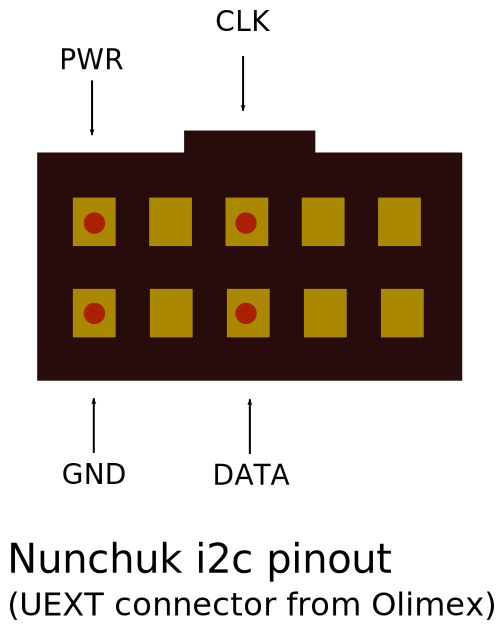
\includegraphics[width=4cm]{labs/buildroot-rootfs/nunchuk-pinout.pdf}
\end{center}

Connect the nunchuk pins:
\begin{itemize}
\item The \code{GND} pin to P9 pins 1 or 2 (\code{GND})
\item The \code{PWR} pin to P9 pins 3 or 4 (\code{DC_3.3V})
\item The \code{CLK} pin to P9 pin 17 (\code{I2C1_SCL})
\item The \code{DATA} pin to P9 pin 18 (\code{I2C1_SDA})
\end{itemize}

\begin{center}
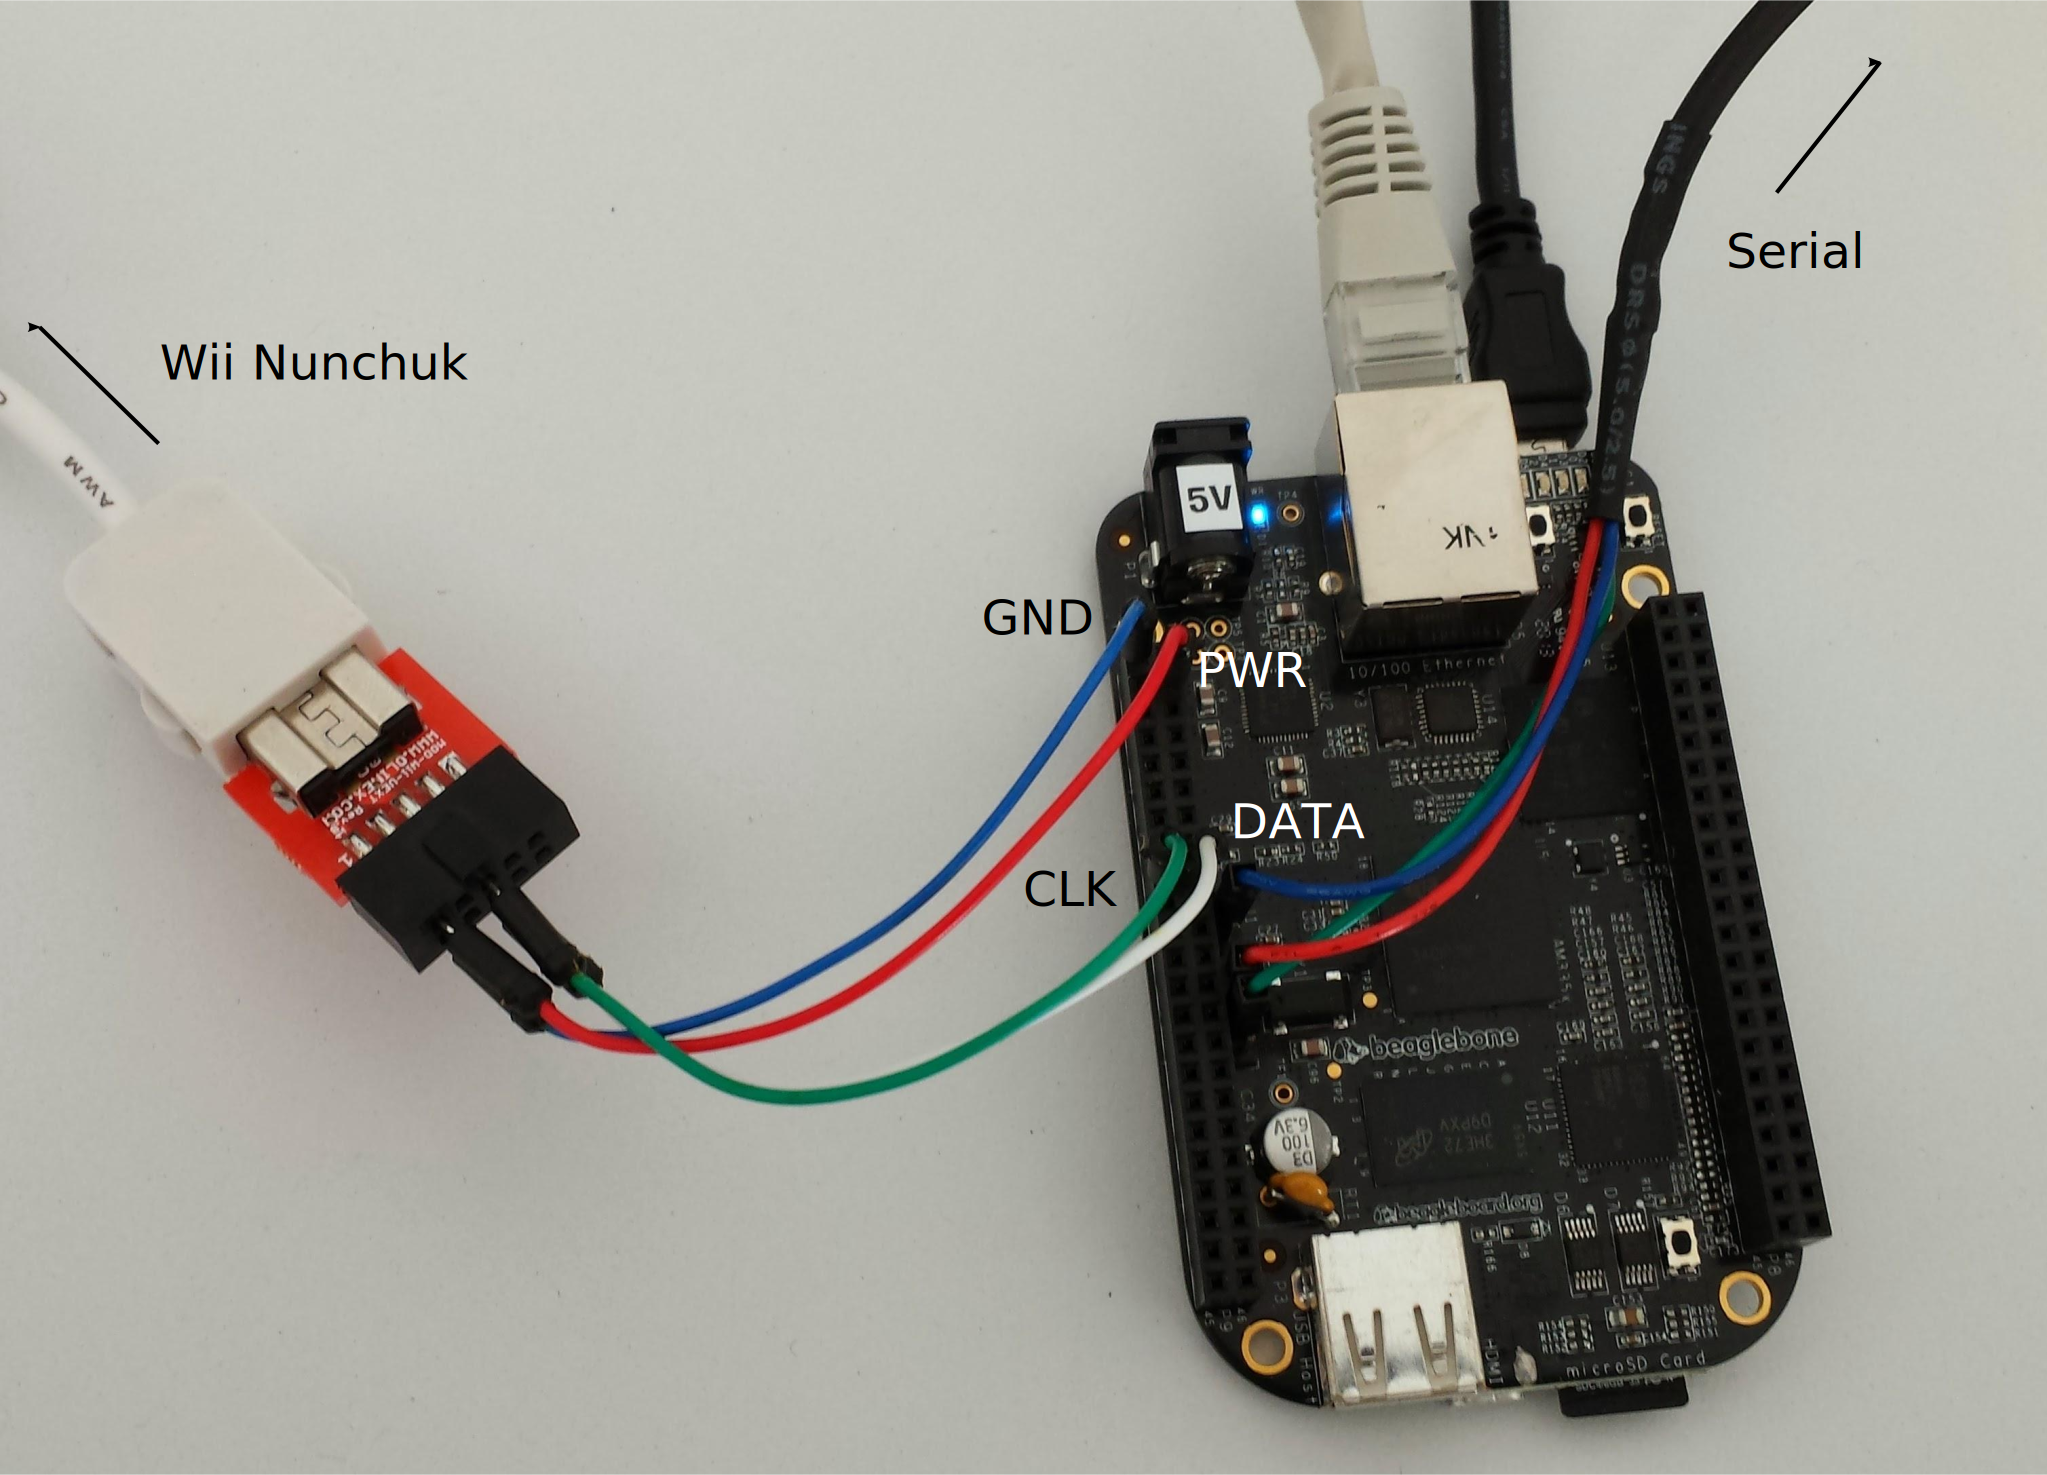
\includegraphics[width=12cm]{labs/buildroot-rootfs/bbb-connect-nunchuk.pdf}
\end{center}

\section{Test the {\em nunchuk}}

Reflash your system, both the {\em Device Tree}, Linux kernel image
and root filesystem, and boot it.

In the kernel boot log, you should see a message like:

\begin{verbatim}
input: Wiichuck expansion connector as /devices/platform/ocp/4802a000.i2c/i2c-1/1-0052/input/input0
\end{verbatim}

You can also explore {\em sysfs}, and see that your Nunchuk device is
handled by the system:

\begin{verbatim}
cat /sys/bus/i2c/devices/1-0052/name
\end{verbatim}

Now, to get the raw events coming from the Nunchuk, you can do:

\begin{verbatim}
cat /dev/input/event0
\end{verbatim}

or, if you prefer to see hexadecimal values instead of raw binary:

\begin{verbatim}
cat /dev/input/event0 | hexdump -C
\end{verbatim}

You should see events when moving the Nunchuk (it has an
accelerometer), when moving the joystick and pushing the buttons.

\section{Add and use {\em input-tools}}

Since the raw events from the Nunchuk are not very convenient to read,
let's install an application that will decrypt the raw input events
and display them in a more human readable format: \code{evtest}.

Enable this package in Buildroot, restart the build, reflash the root
filesystem and reboot the system. Now you can use \code{evtest}:

\begin{verbatim}
evtest /dev/input/event0
\end{verbatim}

\section{Generate a {\em defconfig}}

Now that our system is already in a good shape, let's make sure its
configuration is properly saved and cannot be lost. Go in
\code{menuconfig}, and in the \code{Build options} menu. There is an
option called \code{Location to save buildroot config} which indicates
where Buildroot will save the {\em defconfig} file generated by
\code{make savedefconfig}. Adjust this value to
\code{$(TOPDIR)/configs/felabs_defconfig}.

Then, exit \code{menuconfig}, and run:

\begin{verbatim}
make savedefconfig
\end{verbatim}

Read the file \code{configs/felabs_defconfig} generated in the
Buildroot sources. You will see the values for all the options for
which we selected a value different from the default. So it's a very
good summary of what our system is.

Identify the options related to the following aspects of the system:

\begin{itemize}
\item The architecture specification
\item The toolchain definition
\item The system configuration
\item The Linux kernel related configuration
\item The selection of packages
\item The U-Boot related configuration
\end{itemize}

\section{Testing a full rebuild}

To make sure that we are able to rebuild our system completely, we'll
start a build from scratch. And to learn something new, we'll use {\em
  out of tree} build.

To do so, create a build directory anywhere you want, and move inside
this directory:

\begin{verbatim}
mkdir ~/felabs/buildroot-build/
cd ~/felabs/buildroot-build/
\end{verbatim}

Now, we will load the \code{felabs_defconfig}:

\begin{verbatim}
make -C ~/felabs/buildroot/ O=$(pwd) felabs_defconfig
\end{verbatim}

Let's explain a little bit what happens here. By using
\code{-C ~/felabs/buildroot/}, we in fact tell \code{make} that the
\code{Makefile} to analyze is not in the current directory, but in the
directory passed as the \code{-C} argument. By passing \code{O=}, we
tell Buildroot where all the output should go: by default it goes in
\code{output/} inside the Buildroot sources, but here we override that
with the current directory (\code{$(pwd)}).

This command will have two main effects:

\begin{enumerate}

\item It will load the \code{felabs_defconfig} as the current
  configuration. After running the command, read the file named
  \code{.config}. It's much longer than the {\em defconfig}, because
  it contains the values for all options.

\item It will create a minimal \code{Makefile} in this output
  directory, which will allow us to avoid doing the \code{make -C
    ... O=...} dance each time.

\end{enumerate}

Now that this is done, start the build. You can again save the build
log:

\begin{verbatim}
make 2>&1 | tee build.log
\end{verbatim}

